% !TEX root = ../../I4PRJ, Grp3 - Rapport.tex
\chapter{Specifikation og Analyse}\label{SpecOgAnalyse}
Afsnittet beskriver specifikations- og analysearbejdet. Specifikationsarbejdet begyndte med analyse af projektformulering. Analysen bestod af at løse de problemstillinger, som projektformuleringen rejser vha. user stories. User stories, som er resultatet af analyse arbejdet, ses i det tidligere afsnit~\ref{FunkKrav}. Gruppen bestemte at have fokus på at lave de dele, som har mest værdig for slutbrugeren af systemet. User stories blev prioriteret ved en MoSCoW analyse, som også fremgår i tabel~\ref{table:functional}. Til at danne overblik over systemets domæner, foretog gruppen en domæneanalyse\todo{ref til metoden domæneanalyse, som ikke findes} af user stories. Resultatet af analysen ses på figur~\ref{fig:domainmodel}.

\begin{figure}
	\centering
	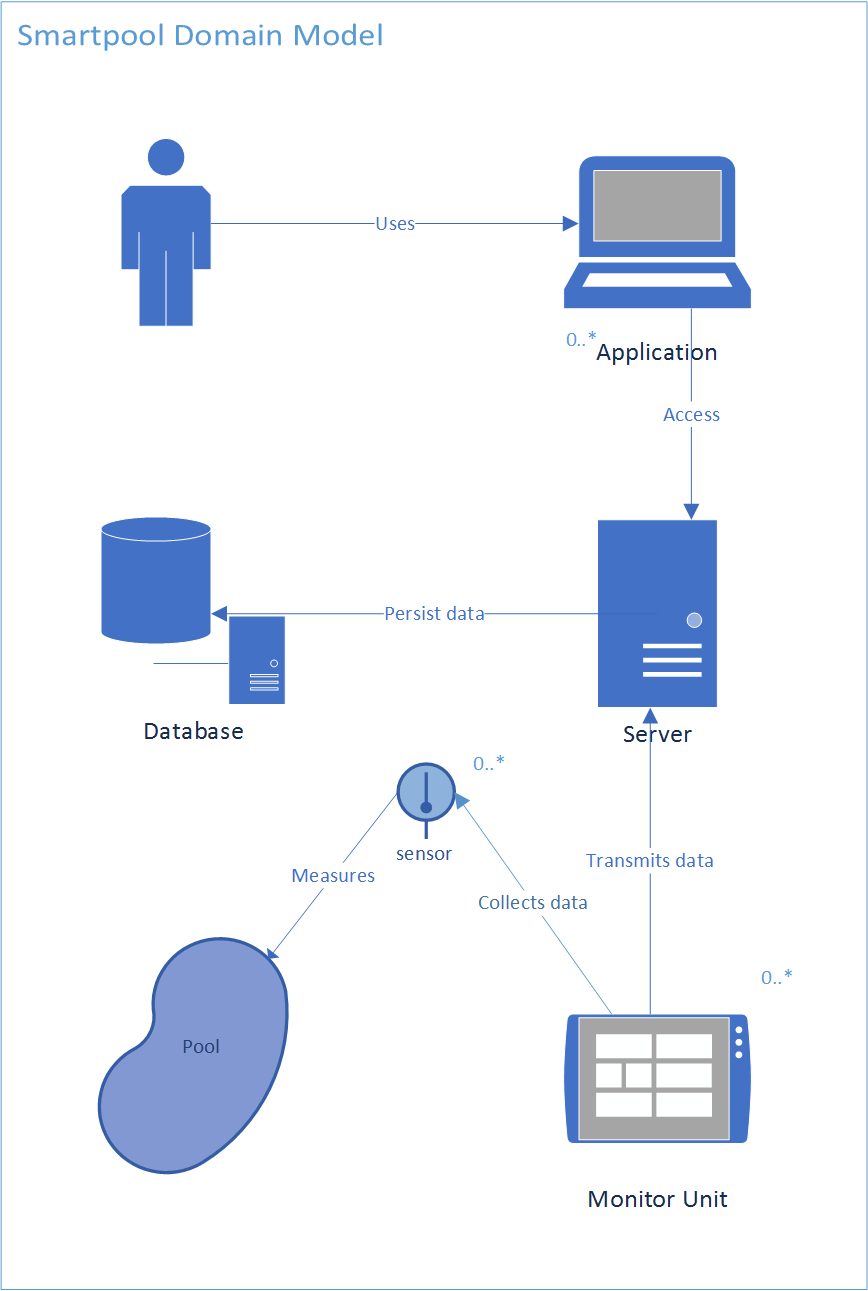
\includegraphics[width=0.7\linewidth]{figs/DomainModelGraphic}
	\caption{Domænemodel for systemet}
	\label{fig:domainmodel}
\end{figure}

For en domænebeskrivelse se dokumentationen afsnit Domænebeskrivelser under Kravspecifikation.

Smartpool projektet afgrænses til at være foruden dataopsamlingsdelen. Figur~\ref{fig:domainmodelboundary} viser det endelige domæne projektet omhandler.

\begin{figure}
	\centering
	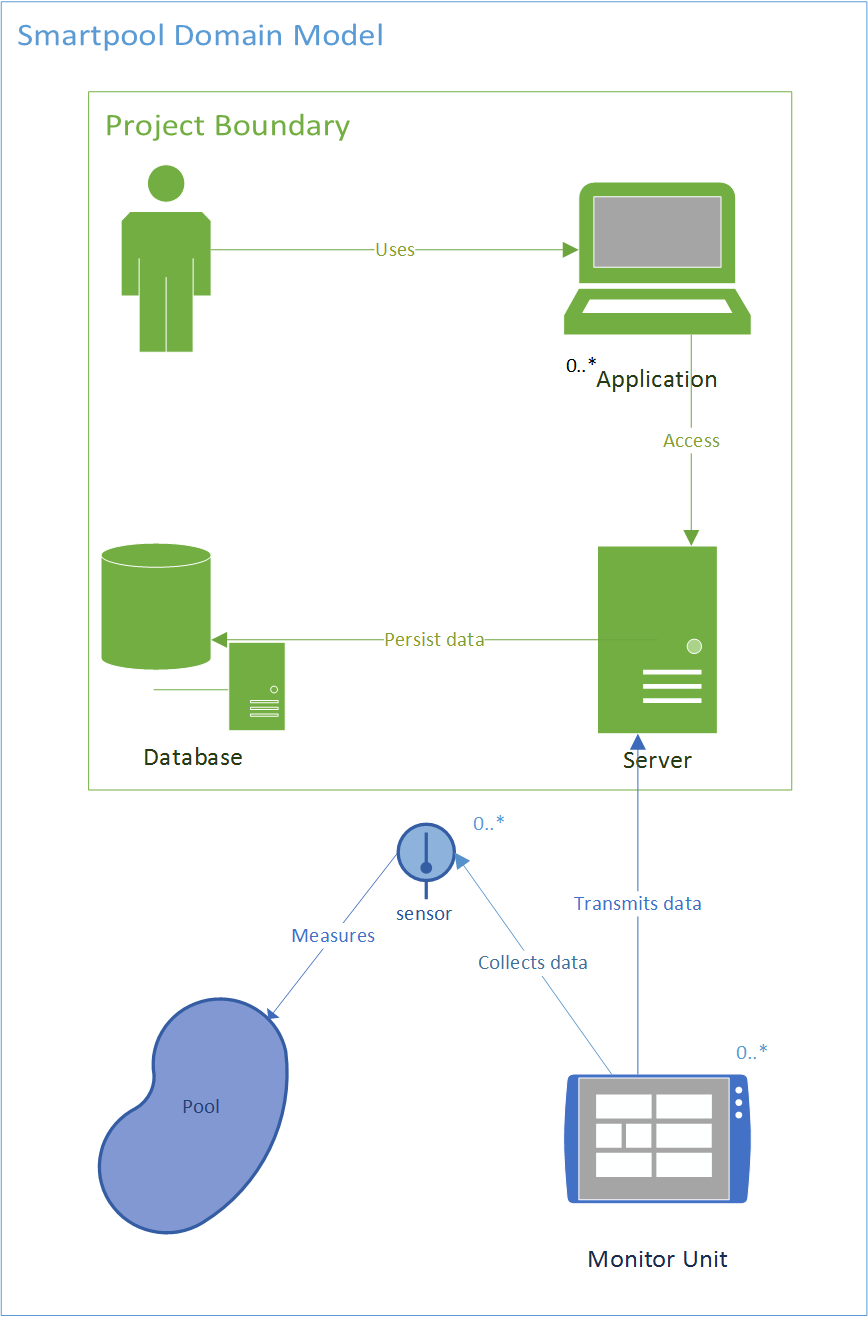
\includegraphics[width=0.7\linewidth]{figs/ProjectBoundary}
	\caption{Domænemodel for systemet}
	\label{fig:domainmodelboundary}
\end{figure}